% !TeX root = ../build/main.tex

The Vocdoni Ballot Protocol defines a simple and efficient mechanism for casting and tallying votes in any type of election or collective decision-making process. Each voting process consists of one or more fields, and voters are required to provide a response for each field in their ballot.

The responses in the ballot are represented as a sequence of natural numbers, each corresponding to the voter’s choice for the respective field. Results are accumulated into a single array. Each position in the array corresponds to the sum of all votes cast for that field across all voters.

The ballot protocol is defined by a set of configurable variables that dictate how votes must be cast. This way the protocol can accommodate a wide range of voting processes and behaviors.

\begin{enumerate}
	\item \textbf{maxCount}: Defines the maximum number of fields in a ballot (max 64).
	\item \textbf{maxValue}: The maximum allowable value for any field in a ballot (if greater than 0).
	\item \textbf{minValue}: The minimum allowable value for any field in a ballot (default 0).
	\item \textbf{uniqueValues}: Specifies whether voters can select the same value multiple times within a ballot (default false).
	\item \textbf{maxTotalCost}: Limits the sum of all field values in a ballot (if greater than 0).
	\item \textbf{minTotalCost}: Specifies a minimum required total sum of field values in a ballot (default 0)
	\item \textbf{costExponent}: Defines the exponent used to calculate the "cost" of votes for each field (default 1
\end{enumerate}

\begin{figure}[H]
	\centering
	\fbox{
		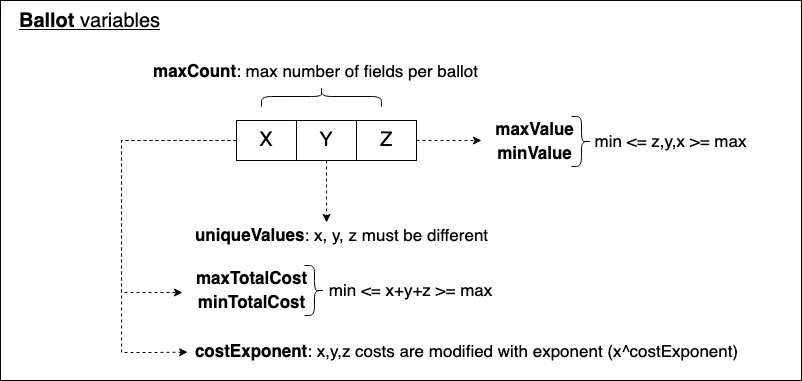
\includegraphics[scale = 0.4, draft = false]{\figs/ballot-variables.png}}
\end{figure}

\textbf{Example 1: Rating Candidates}

Consider a voting process where voters are asked to rate three candidates: Lennon, Hendrix, and Joplin. Voters rate each candidate from 0 to 5 stars, and each vote is represented as an array where each position corresponds to the candidate’s rating.

Configuration:

\begin{itemize}
	\item \texttt{maxCount}: 3
	\item \texttt{maxValue}: 5
	\item \texttt{uniqueValues}: Yes
\end{itemize}

Ballots:

\begin{itemize}
	\item Vote 1: \texttt{[3, 2, 5]} (3 stars for Lennon, 2 stars for Hendrix, 5 stars for Joplin)
	\item Vote 2: \texttt{[4, 3, 2]}
	\item Vote 3: \texttt{[2, 4, 5]}
\end{itemize}

After accumulating the votes:

\begin{itemize}
	\item Results Array: \texttt{[3+4+2, 2+3+4, 5+2+5] = [9, 9, 12]}\\
	Lennon received 9 points, Hendrix received 9 points, and Joplin received 12 points.
\end{itemize}

\textbf{Example 2: Quadratic Voting for Resource Allocation}

In a scenario where voters distribute a fixed number of credits across different options (e.g., selecting funding levels for NGOs), the ballot allows voters to assign multiple points, but the cost of casting multiple votes for a single option increases quadratically.

Configuration:

\begin{itemize}
	\item \texttt{maxCount}: 4
	\item \texttt{maxTotalCost}: 12 (credits)
	\item \texttt{costExponent}: 2 (quadratic)
\end{itemize}

Ballots:

\begin{itemize}
	\item Vote 1: \texttt{[2, 2, 2, 0]}
	\item Vote 2: \texttt{[1, 1, 3, 1]}
	\item Vote 3: \texttt{[0, 2, 1, 2]}
\end{itemize}


After accumulating the votes:


\begin{itemize}
	\item Results Array: \texttt{[2+1+0, 2+1+2, 2+3+1, 0+1+2] = [3, 5, 6, 3]} \\
	Each position in the array represents the total sum of credits allocated to each NGO.
\end{itemize}

